% bei Standalone in documentclass noch:
% \RequirePackage{luatex85}

\documentclass[captions=tableheading, titlepage= firstiscover, parskip = half , bibliography=totoc]{scrartcl}
%paper = a5 für andere optinen
% titlepage= firstiscover
% bibliography=totoc für bibdateien
% parskip=half  Veränderung um Absätze zu verbessern

\usepackage{scrhack} % nach \documentclass
\usepackage[aux]{rerunfilecheck}
\usepackage{polyglossia}
\usepackage[style=numeric, backend=biber]{biblatex} % mit [style = alphabetic oder numeric] nach polyglossia
\addbibresource{lit.bib}
\setmainlanguage{german}

\usepackage[autostyle]{csquotes}
\usepackage{amsmath} % unverzichtbare Mathe-Befehle
\usepackage{amssymb} % viele Mathe-Symbole
\usepackage{mathtools} % Erweiterungen für amsmath
\usepackage{fontspec} % nach amssymb
% muss ins document: \usefonttheme{professionalfonts} % für Beamer Präsentationen
\usepackage{longtable}

\usepackage[
math-style=ISO,    % \
bold-style=ISO,    % |
sans-style=italic, % | ISO-Standard folgen
nabla=upright,     % |
partial=upright,   % /
]{unicode-math} % "Does exactly what it says on the tin."
\setmathfont{Latin Modern Math}
% \setmathfont{Tex Gyre Pagella Math} % alternativ

\usepackage[
% die folgenden 3 nur einschalten bei documenten
locale=DE,
separate-uncertainty=true, % Immer Fehler mit ±
per-mode=symbol-or-fraction, % m/s im Text, sonst \frac
]{siunitx}

% alternativ:
% per-mode=reciprocal, % m s^{-1}
% output-decimal-marker=., % . statt , für Dezimalzahlen

\usepackage[
version=4,
math-greek=default,
text-greek=default,
]{mhchem}

\usepackage[section, below]{placeins}
\usepackage{caption} % Captions schöner machen
\usepackage{graphicx}
\usepackage{grffile}
\usepackage{subcaption}

% \usepackage{showframe} Wenn man die Ramen sehen will

\usepackage{float}
\floatplacement{figure}{htbp}
\floatplacement{table}{htbp}

\usepackage{mhchem} %chemische Symbole Beispiel: \ce{^{227}_{90}Th+}


\usepackage{booktabs}

 \usepackage{microtype}
 \usepackage{xfrac}

 \usepackage{expl3}
 \usepackage{xparse}

 % \ExplSyntaxOn
 % \NewDocumentComman \I {}  %Befehl\I definieren, keine Argumente
 % {
 %    \symup{i}              %Ergebnis von \I
 % }
 % \ExplSyntaxOff

 \usepackage{pdflscape}
 \usepackage{mleftright}

 % Mit dem mathtools-Befehl \DeclarePairedDelimiter können Befehle erzeugen werden,
 % die Symbole um Ausdrücke setzen.
 % \DeclarePairedDelimiter{\abs}{\lvert}{\rvert}
 % \DeclarePairedDelimiter{\norm}{\lVert}{\rVert}
 % in Mathe:
 %\abs{x} \abs*{\frac{1}{x}}
 %\norm{\symbf{y}}

 % Für Physik IV und Quantenmechanik
 \DeclarePairedDelimiter{\bra}{\langle}{\rvert}
 \DeclarePairedDelimiter{\ket}{\lvert}{\rangle}
 % <name> <#arguments> <left> <right> <body>
 \DeclarePairedDelimiterX{\braket}[2]{\langle}{\rangle}{
 #1 \delimsize| #2
 }

\setlength{\delimitershortfall}{-1sp}

 \usepackage{tikz}
 \usepackage{tikz-feynman}

 \usepackage{csvsimple}
 % Tabellen mit \csvautobooktabular{"file"}
 % muss in table umgebung gesetzt werden


% \multicolumn{#Spalten}{Ausrichtung}{Inhalt}

\usepackage{hyperref}
\usepackage{bookmark}
\usepackage[shortcuts]{extdash} %nach hyperref, bookmark

\newcommand{\ua}[1]{_\symup{#1}}
\newcommand{\su}[1]{\symup{#1}}


\title{Versuch 207}
\subtitle{Das Kugelfall-Viskosimeter nach Höppler}
\author{Sebastian Pape\\
        sepa@gmx.de \and
        Jonah Nitschke\\
        lejonah@web.de}
\date{Durchführung: 22.11.2016\\
      Abgabe: 29.11.2016}

\begin{document}

\maketitle
\tableofcontents
\newpage

\section{Einführung}

Der Versuch zielt darauf ab die Temperaturabhängigkeit der dynamischen Viskosität von destilliertem
Wasser, mit Hilfe der Kugelfallmethode zu bestimmen. Zunächst werden die theoretischen Grundlagen
erklärt, danach wird die Durchführung und der Aufbau erläutert. Daraufhin folgt die Auswertung der Versuchsergerbnisse
mit abschließender Diskussion.

\section{Theorie}

\subsection{Innere Reibung}

Sobald ein Körper durch ein Medium bewegt wird, entsteht innere Reibung. Die Stärke dieser Reibung hängt von der Beschaffenheit
des Umgebungsmediums ab und wird als dynamische Viskosität oder auch Zähigkeit bezeichnet.
In dem Versuch wurde eine Kugel, mit Radius $r$ durch destilliertes Wasser bewegt. Die Reibungskraft, die der Bewegung
entgegengerichtet ist, lässt sich über das \emph{Stokessche Gesetz} bestimmen.
\begin{equation}
  \label{eqn:Stokes}
  F_R = 6\pi r \eta v
\end{equation}
Dabei ist $\eta$ die dynamische Viskosität und $v$ die Geschwindigkeit der Kugel. Die \emph{Stokes Gleichung} gilt nur für laminare
Strömungen, was bedeutet, dass die Ausdehnung der Flüssigkeit hinreichend groß sein muss, wodurch Wirbelbildungen verhindert werden.
Die Kugel wird in dem Versuch durch ein Rohr mit leicht größerem Durchmesser als dem der Kugel fallen gelassen.
Die erreichten Fallgeschwindigkeit der Kugel durch das Medium sind darüberhinaus hinreichend gering, sodass
alle Voraussetzungen für die Gültigkeit von Gleichung \eqref{eqn:Stokes} gegeben sind.
Wenn die Kugel in einer viskosen Flüssigkeit fällt, wirken zum einem ihre Gewichtskrat $F_g$, die Reibungskraft der Flüssigkeit $F_R$
und der Auftrieb $F_A$. Die Auftriebskraft ist wie die Reibungskraft der Bewegungsrichtung entgegengerichtet.
Die Reibungskraft nimmt mit zunehmender Geschwindigkeit der Kugel zu. Dies bedeutet, dass sich ein Kräftegleichgewicht zwischen
$F_g$ und $F_R$ einstellt, wodurch sich eine konstante Fallgeschwindigkeit ergibt.
Die Zähigkeit der Flüssigkeit lässt sich über das empirische gefundene Gesetz \eqref{eqn: dyn. Viskosität} bestimmen.
\begin{equation}
  \label{eqn: dyn. Viskosität}
  \eta = K(\rho_K - \rho_{Fl}) \cdot t
\end{equation}
Wobei $K$ eine Apparaturkonstante, $\rho_K$ die Dichte der Kugel, $\rho_{Fl}$ die Dichte der Umgebungsflüssigkeit und $t$ die Fallzeit ist.
Die Apparaturkonstante enthält sowohl Informationen über die Fallhöhe, als auch über die Kugelgeometrie.

\subsection{Temperaturabhängigkeit der Viskosität}

Die Temperaturabhängigkeit der dynamischen Viskosität lässt sich mit Hilfe der \emph{Andradeschen Gleichung} bestimmen, die da lautet
\begin{equation}
  \eta(T) = A \exp\left(\frac{B}{T}\right).
\end{equation}
$A$ und $B$ sind dabei Konstanten, die über eine Ausgleichsrechung bestimmt werden können.

\subsection{Reynolds Zahl}

Die \emph{Stokes Gleichung} ist nur für laminare Strömungen gültig. Das Strömungsverhalten einer laminaren Strömung charakterisiert sich
dadurch, dass die Strömugslinien immer nebeneinander verlaufen und keine Wirbel ausbilden. Sobald eine bestimmte Strömungsgeschwindigkeit
erreicht ist, ändert sich das Strömungsverhalten des Fluides hin zu einer trubulenten Strömung. Also einer Strömung, in der die Strömungslinien
Wirbel ausbilden. Die \emph{Reynolds Zahl} $Re$ ist eine Kenngröße, anhand der das Strömungsverhalten von Flüssigkeiten charakterisiert werden kann.
Sie ist definiert als,
\begin{equation}
  \label{eqn:Reynolds Zahl}
  Re = \frac{ \rho_{w} \cdot v \cdot d}{\eta}
\end{equation}

wobei $\rho_{w}$ die Dichte der Flüssigkeit, $v$ die Fließgeschwindigkeit und $d$ der Kugeldurchmesser ist.
Empirisch wurde gefunden, dass eine Flüssigkeit mit $Re < 2000$ ein laminares Strömungsverhalten aufweist. Sobald der kritische Wert von $Re < 3000$
überschritten wird, ist ein turbulentes Strömungsverhalten der Flüssigkeit vorzufinden. In dem Grenzbereich von $2000$ bis $3000$ ist das
Verhalten der Flüssigkeit nicht klar definiert und kann zwischen den beiden Strömungsverhalten wechseln.

\section{Durchführung}

Im Folgendem wird die Durchführung des Versuches geschildert.
Zu Beginn des Versuches müssen die Dichten der verwendeten Kugeln ermittelt werden. Die Masse der Kugeln wird mit Hilfe einer Waage und
die Durchmesser mit Hilfe einer Schieblehre gemessen. Danach wird das Kugelfall-Viskosimeter mit Hilfe einer Libelle (siehe Abb. \ref{fig:Aufbau})
justiert. Nun kann die zu untersuchende Flüssigkeit, in diesem Fall destilliertes Wasser und die Kugel in das Viskosimeter gegeben werden.
Es ist darauf zu achten, dass keine Luftblasen an der Rohrinnenseite und der Kugel haften, da durch diese die
Fallzeit unvorhersehbar beeinflusst wird. Insgesamt werden zwei Kugeln mit unterschiedlichen Radien verwendet, wobei jeweil zehn
Fallzeitmessungen bei Raumtemperatur für eine Kugel durchgeführt werden.
Abschließend wird die Messung für die größere der beiden Kugeln mit variierender Temperatur durchgeführt. Es werden für insgesamt
zehn Temperaturen zwei Messungen gemacht. Die Temperaturen sollen zwischen der Raumtemperatur und ca. $\SI{70}{\celsius}$ liegen.


\subsection{Aufbau}

Zur Bestimmung der dynamischen Viskosität von destilliertem Wasser wurde das Kugelfall-Viskosimeter nach Höppler (Abb. \ref{fig:Aufbau}) verwendet.
Das Rohr, durch welches die Kugel fällt ist leicht angewinkelt, sodass die Kugel nicht unkontrolliert hindurchfällt, sondern an der Rohrinnenseite
entlang gleitet.
In die Apparatur kann die zu untersuchende Flüssigkeit, sowie die Kugel über zwei Stopfen eingeführt werden. Das Kugelfall-Viskosimeter ist an ein Thermostat
gekoppelt, durch welches die Rohrumgebendeflüssigkeit temperiert werden kann. Darüberhinaus wird damit die Momentanetemperatur der zu untersuchenden
Flüssigkeit bestimmt. Die in Abb. \ref{fig:Aufbau} dargestellten Messmarken definieren die Fallstrecke der Kugel. Die obere Messmarke ist
$\SI{0,1}{\meter}$ von der unteren entfernt.
Durch ein Schanier kann das Viskosimeter um $\ang{180}$ gedreht werden, um eine weitere Fallgeschwindigkeitsmessung vornehmen zu können.
Die Gewichtskraft der Kugel sollte vor Durchlaufen der ersten Messmarke im Gleichgewicht mit der Reibungskraft der Flüssigkeit sein, da die Zeitmessung
bei konstanter Geschwindigkeit durchzuführen ist.

\begin{figure}
  \centering
  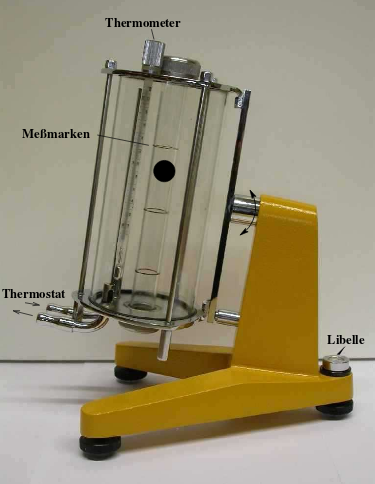
\includegraphics[width=7.50cm, height=9.50cm]{V207_Kugelfall-Viskosimeter_Höppler.png}
  \caption{Kugelfall-Viskosimeter\cite{anleitung01}}
  \label{fig:Aufbau}
\end{figure}

\newpage
\printbibliography
\end{document}
